\chapter{CO\textsubscript{2} and Humidity}
\label{app:co2-humidity}

This appendix supports Chapter~\ref{ch:co2humidity}. It shows the gas joint that failed, the free gas volume of the built chamber, and the CO\textsubscript{2} simulations repeated for that volume.

\section{The Gas Connection}
\label{app:gas-joint}

Figure~\ref{fig:co2-leak-photo} shows the regulator inlet, its nut and the SodaStream adapter face. The failure is described in Section~\ref{sec:co2c-failure}.

\begin{figure}[htbp]
    \centering
    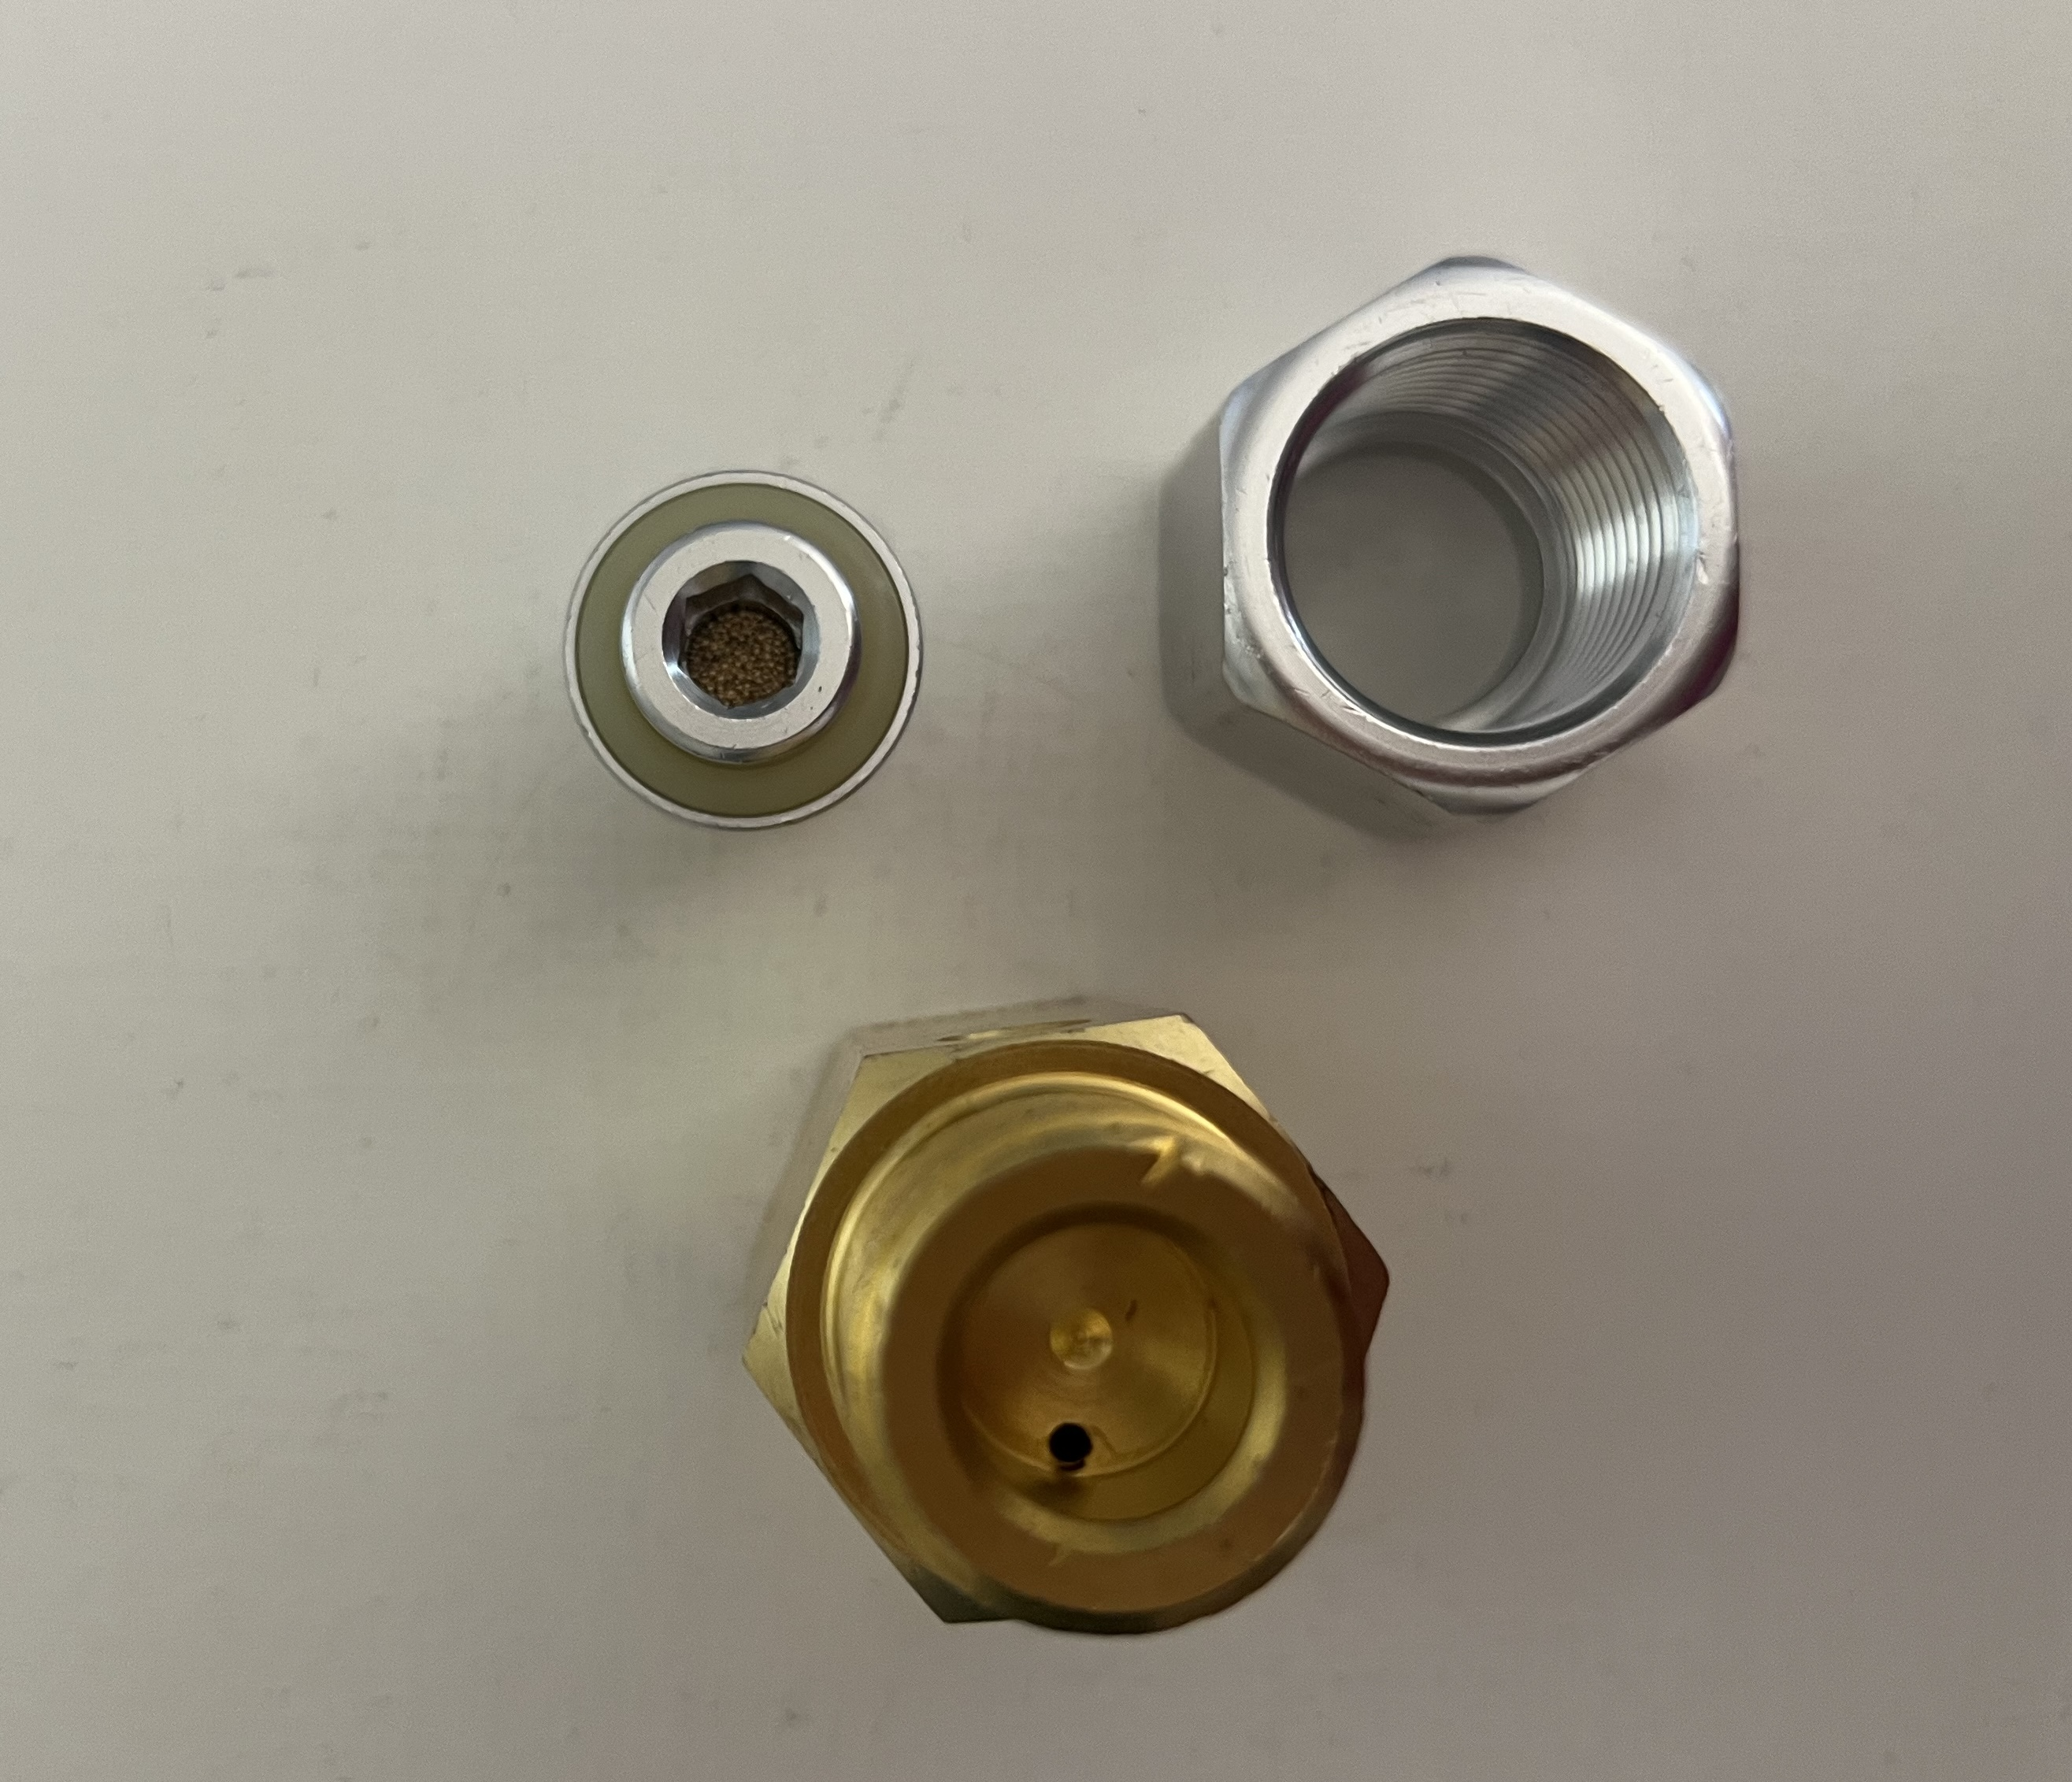
\includegraphics[width=0.6\textwidth]{figs/ch8/CO2 leak.jpeg}
    \caption[The regulator to SodaStream adapter joint]{\textbf{The joint that would not seal.} Left: the regulator inlet, with the filter in the centre of the seal. Right: the nut. Bottom: the face of the SodaStream adapter. The filter cannot enter the adapter, so the seal never reaches the adapter face.}
    \label{fig:co2-leak-photo}
\end{figure}

\FloatBarrier
\section{Free Gas Volume}
\label{app:gas-volume}

The free gas volume used in Section~\ref{sec:co2-params} is the inside volume of the chamber's three stepped sections, minus the volume of the plate (with its wells full) and the two gas sensors (Table~\ref{tab:co2-volume}).

\begin{table}[H]
    \centering
    \caption[Free gas volume of the built chamber]{\textbf{Free gas volume of the built chamber,} from the as-printed geometry. $Z$ is the height above the underside of the base.}
    \label{tab:co2-volume}
    \small
    \begin{tabular}{@{}lccr@{}}
        \toprule
        \textbf{Region} & \textbf{$Z$ range (mm)} & \textbf{Section (mm)} & \textbf{Volume (mm\textsuperscript{3})} \\
        \midrule
        Chamber body      & 0.8 to 26   & $160 \times 118$      & 475\,776 \\
        Top flange        & 26 to 32    & $154 \times 112$      & 103\,488 \\
        Lid aperture      & 32 to 35.8  & $132 \times 90$       & 45\,144 \\
        \midrule
        Enclosed          &             &                       & 624\,408 \\
        Plate, wells full & 0.8 to 13.9 & $127.76 \times 85.48$ & $-143\,065$ \\
        Gas sensors       &             &                       & $-12\,000$ \\
        \midrule
        \textbf{Free gas} &             &                       & \textbf{469\,343} \\
        \bottomrule
    \end{tabular}
\end{table}

\FloatBarrier
\section{CO\textsubscript{2} Simulation for the Built Chamber}
\label{app:co2-sim-built}

The figures below repeat the simulations of Appendix~\ref{app:co2-control-sim} using the built chamber volume of 0.47\,L and the gains in Table~\ref{tab:co2-gains}. Figure~\ref{fig:co2-fill} shows the chamber filling from room air, and Figure~\ref{fig:co2-fill-strategies} compares this with holding the valve open. Figure~\ref{fig:co2-lid} shows the recovery after the lid is opened, with and without the integrator freeze. Figure~\ref{fig:co2-robustness} shows the fill when the leak and flow differ from the design values, Figure~\ref{fig:co2-pulses} shows the valve pulses and ripple at steady state, and Figure~\ref{fig:co2-bode} gives the frequency response.

\begin{figure}[htbp]
    \centering
    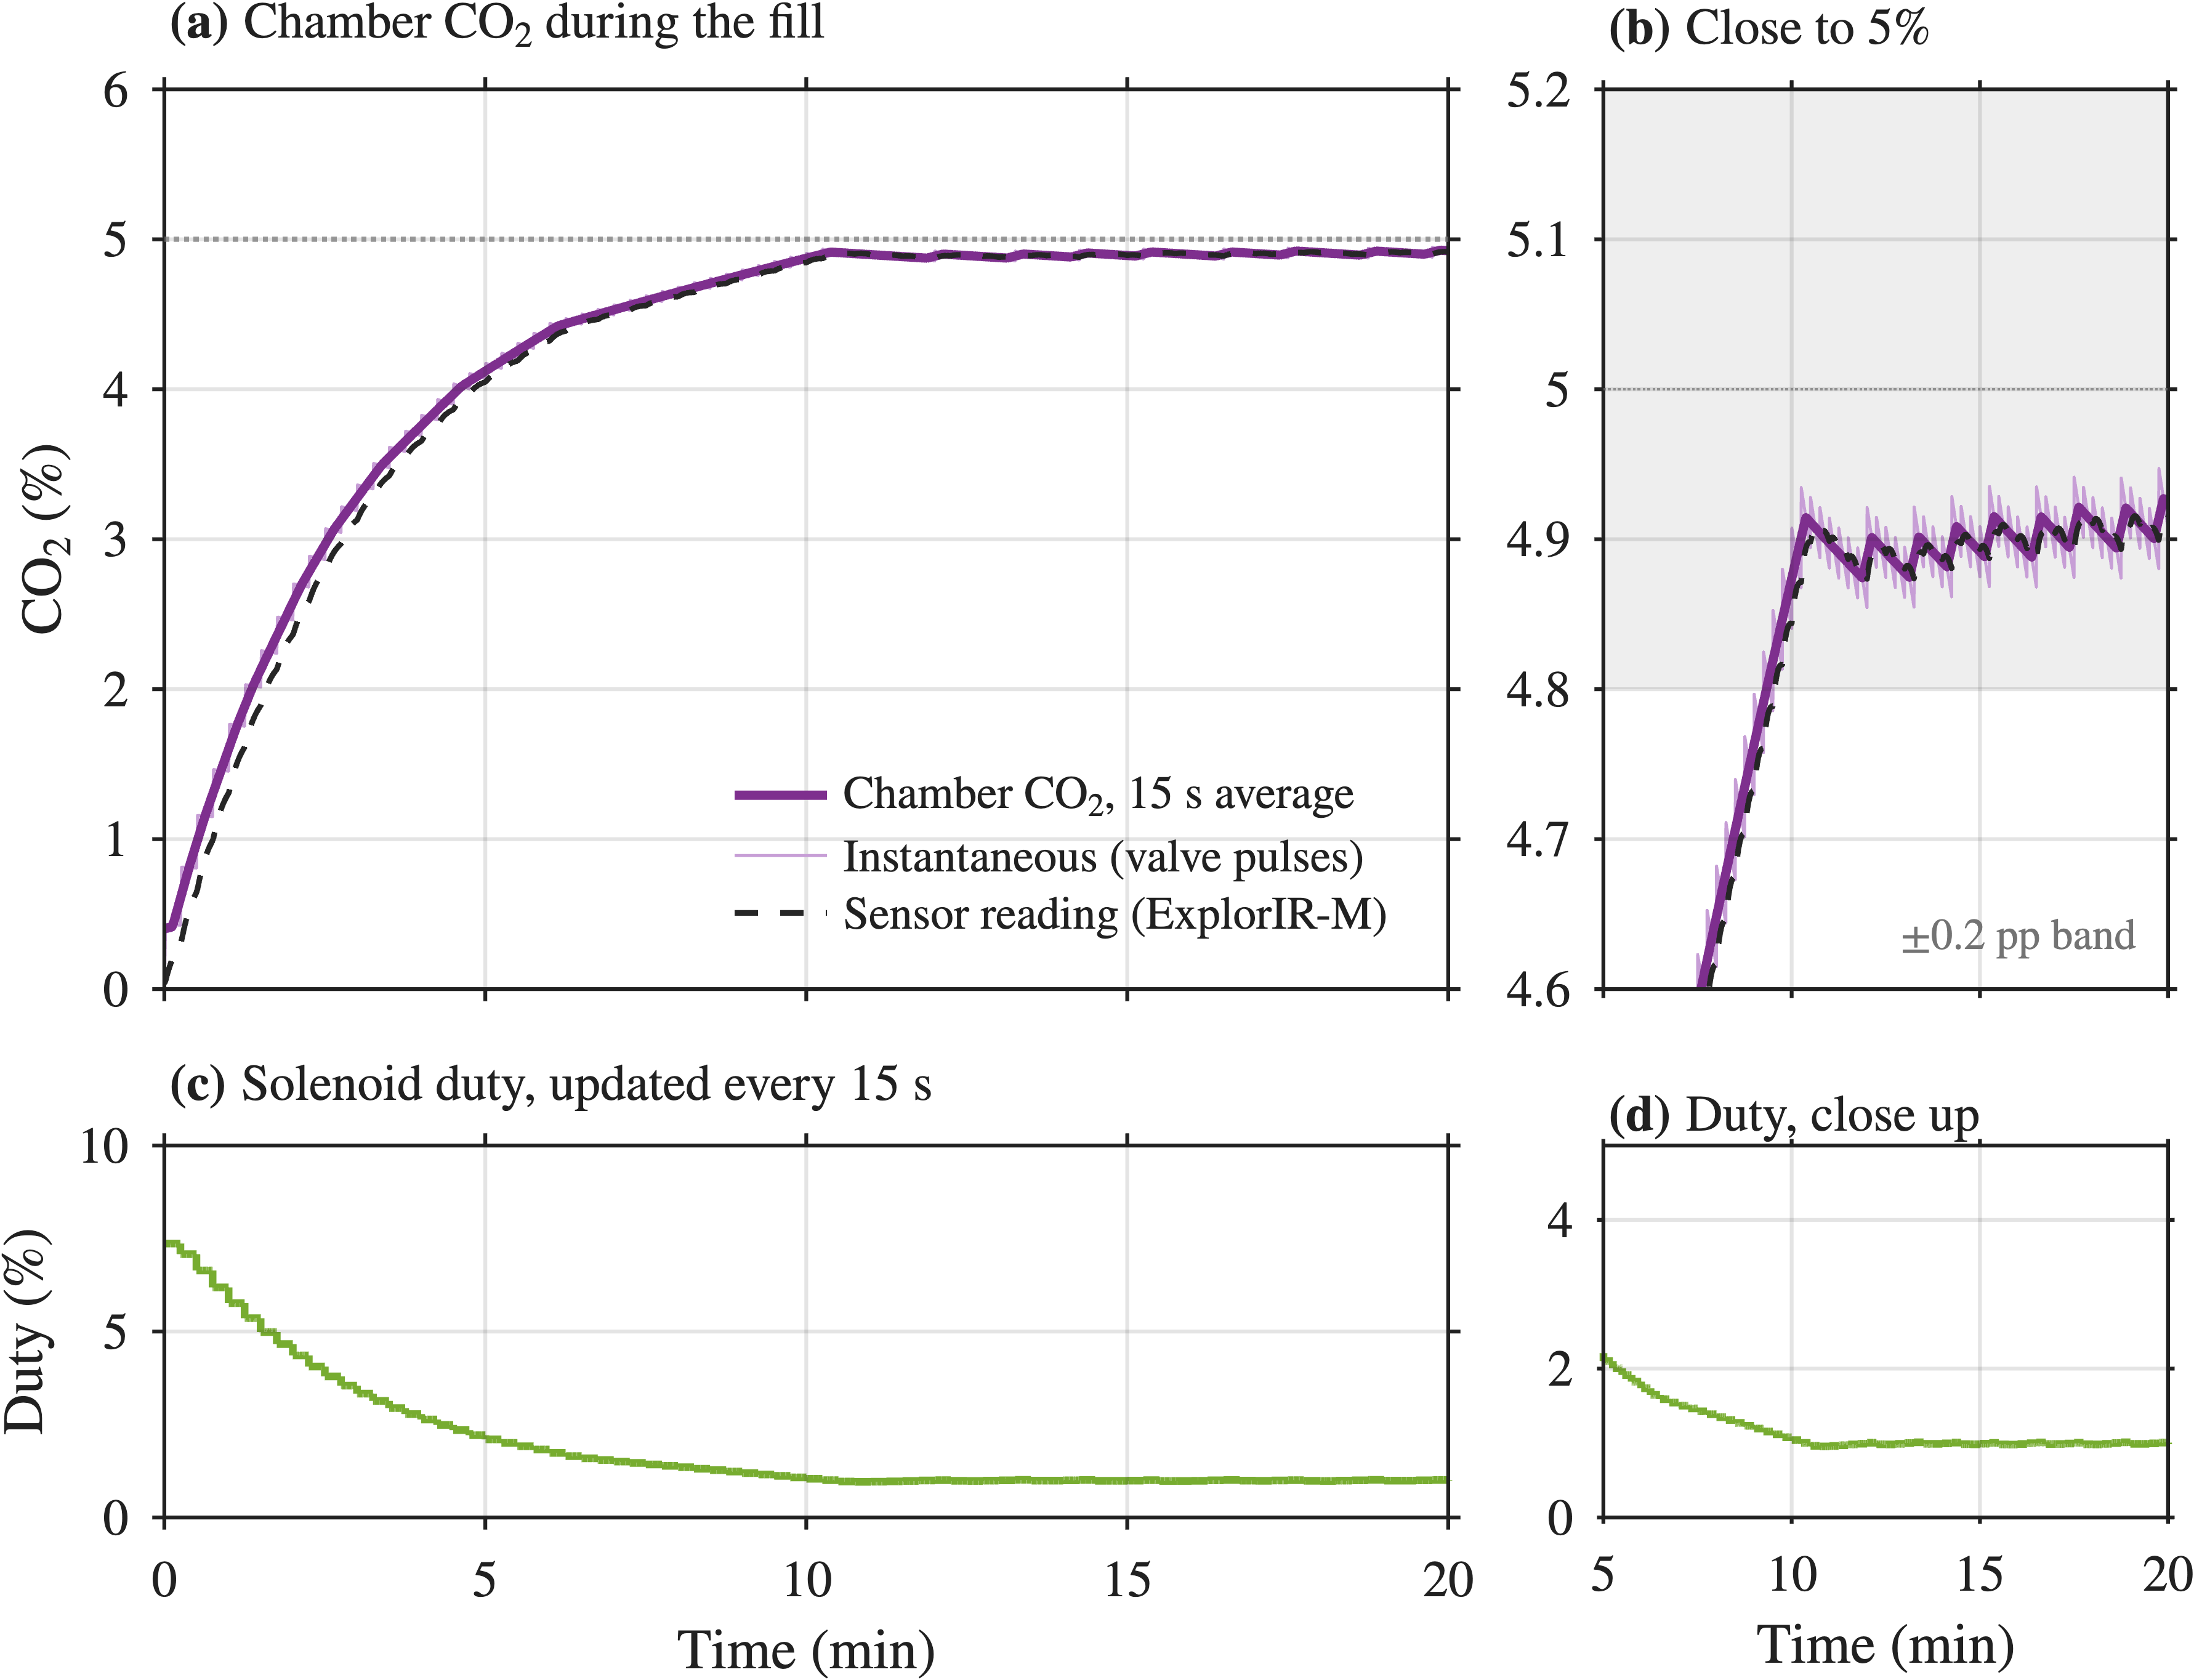
\includegraphics[width=0.74\textwidth,height=0.62\textheight,keepaspectratio]{figs/ch8/NEW_fig_C2_fill.png}
    \caption[Simulated CO\textsubscript{2} fill from room air]{\textbf{Simulated fill from room air with the corrected parameters.} (a) Chamber concentration, the instantaneous trace showing the valve pulses, and the sensor reading. (b) The approach to 5\,\%, with the $\pm$0.2\,pp band shaded. (c, d) Solenoid duty, updated every 15\,s.}
    \label{fig:co2-fill}
\end{figure}

\begin{figure}[htbp]
    \centering
    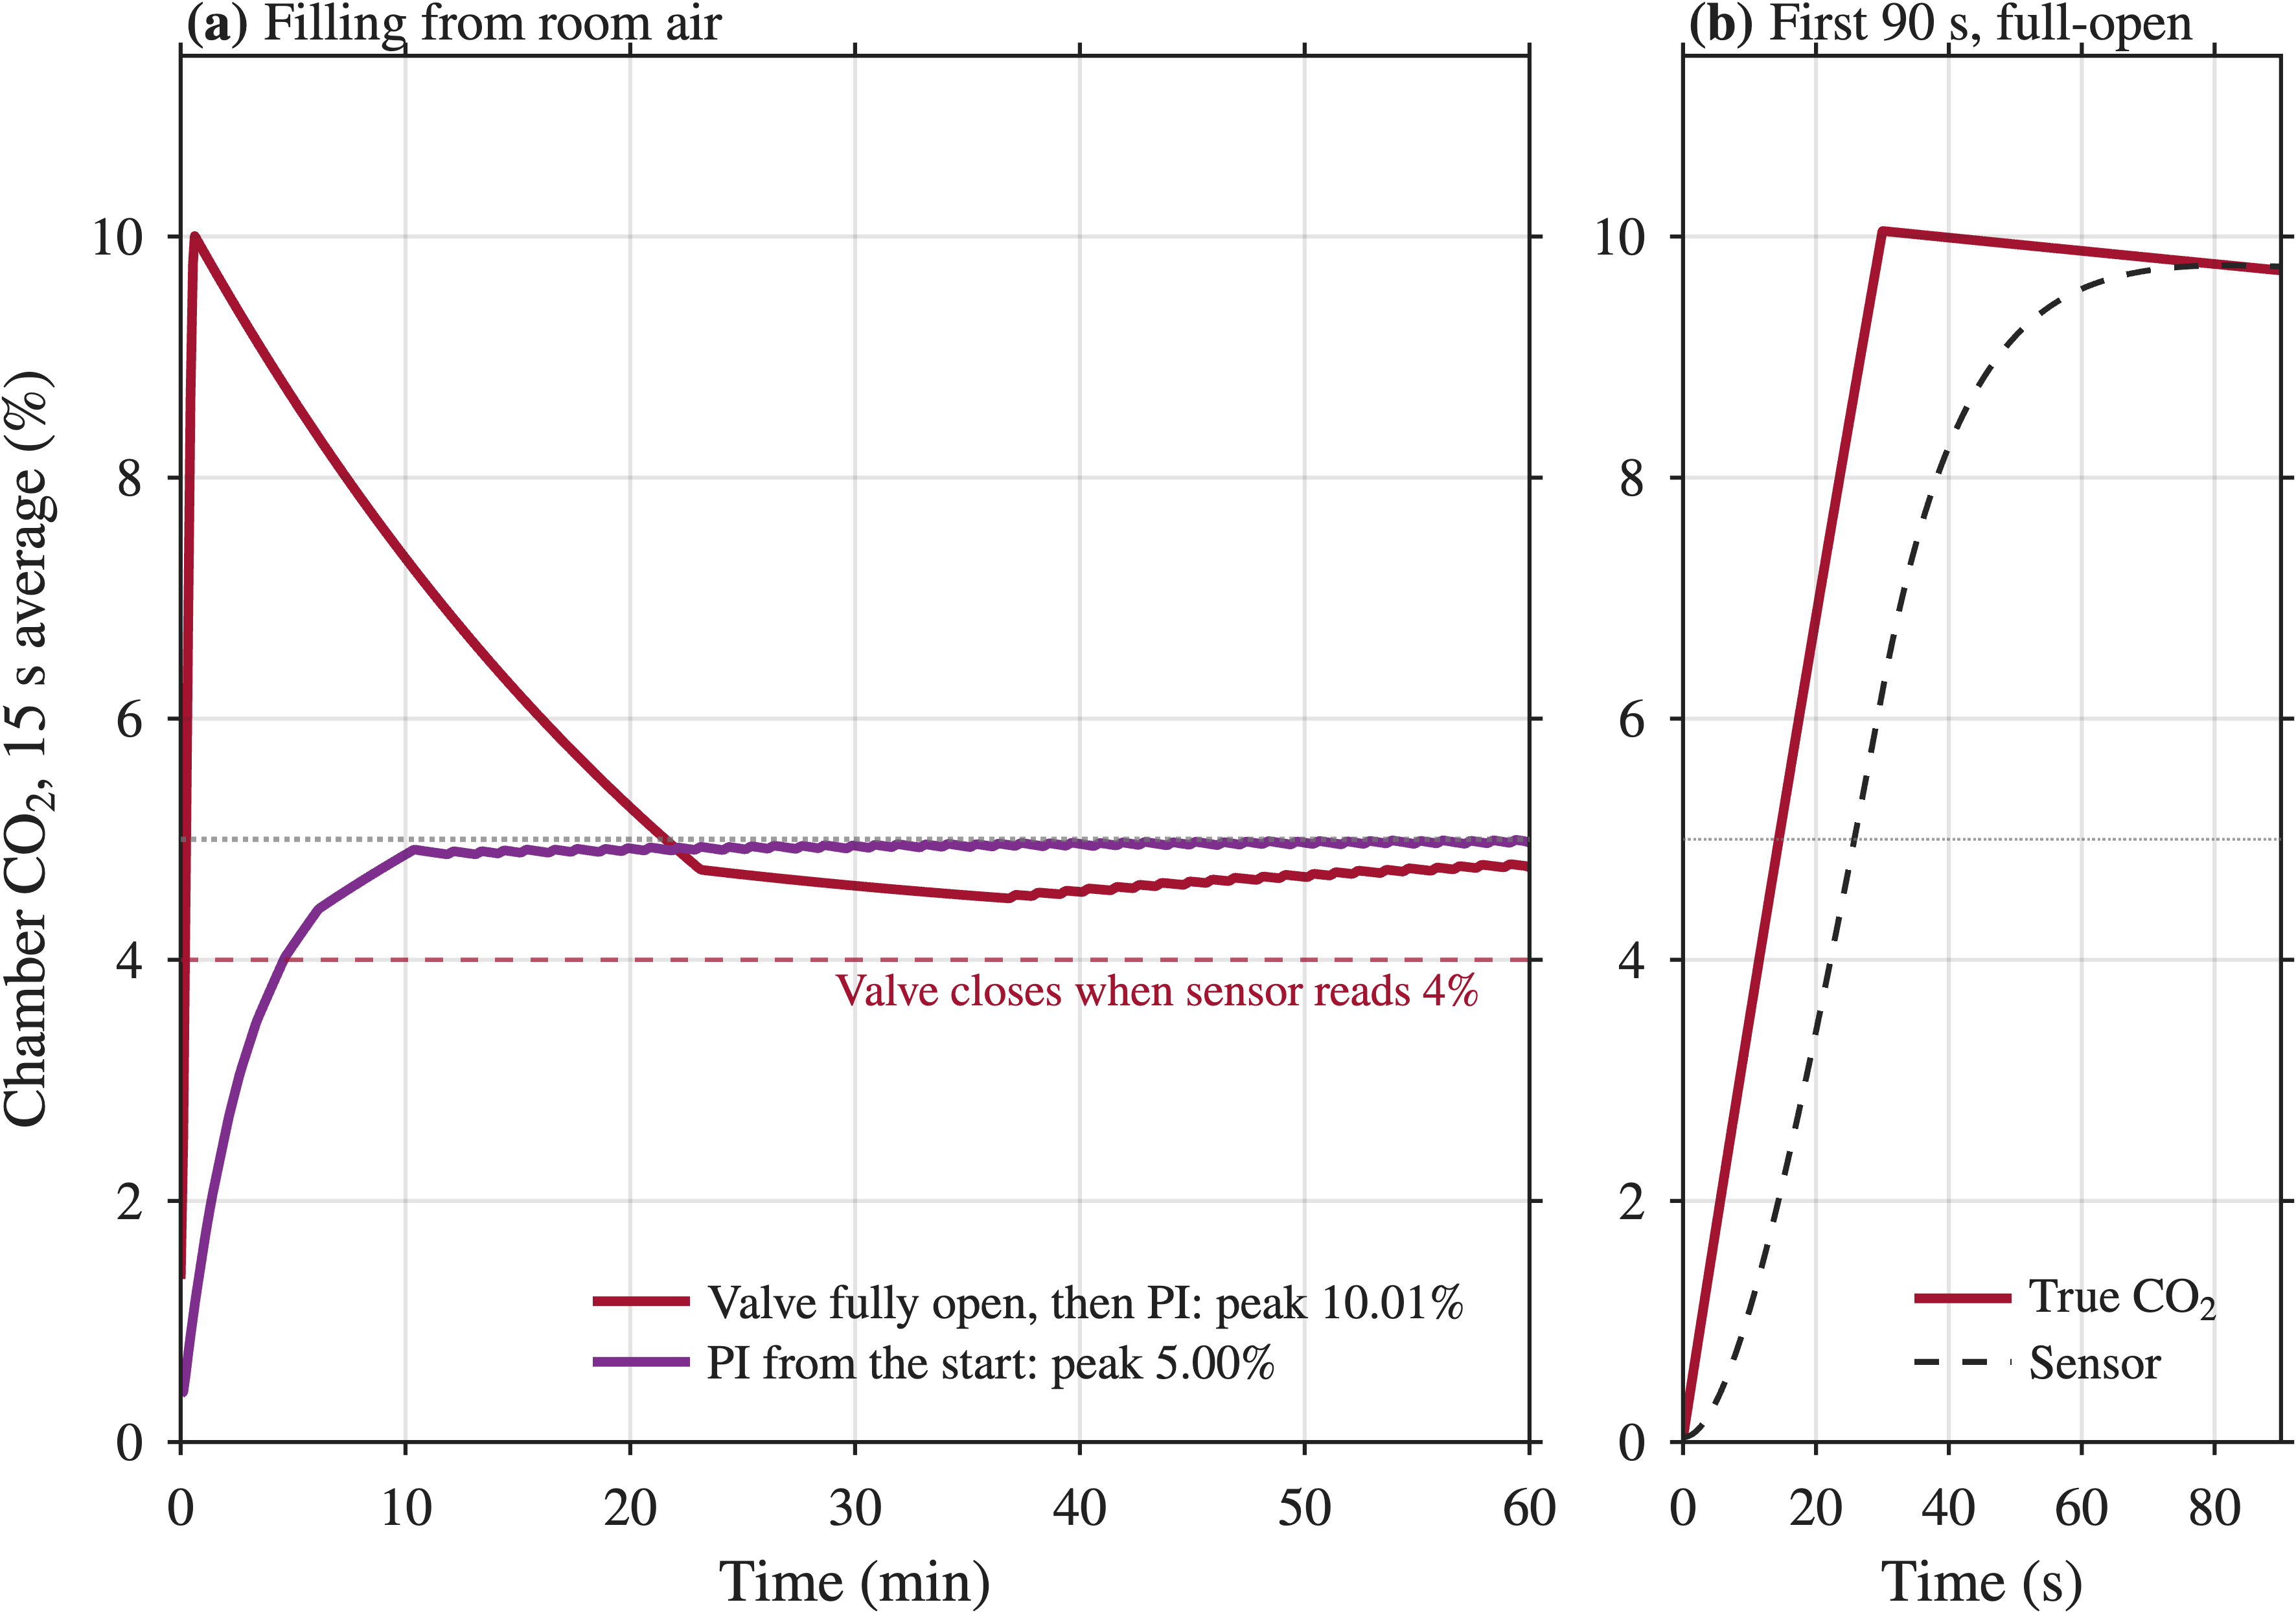
\includegraphics[width=0.74\textwidth,height=0.62\textheight,keepaspectratio]{figs/ch8/NEW_fig_C3_fill_strategies.png}
    \caption[CO\textsubscript{2} fill strategies]{\textbf{Holding the valve open fills past the setpoint.} (a) PI from the start against valve fully open until the sensor reads 4\,\%. (b) The first 90\,s, showing the sensor lagging the chamber during the fast fill.}
    \label{fig:co2-fill-strategies}
\end{figure}

\begin{figure}[htbp]
    \centering
    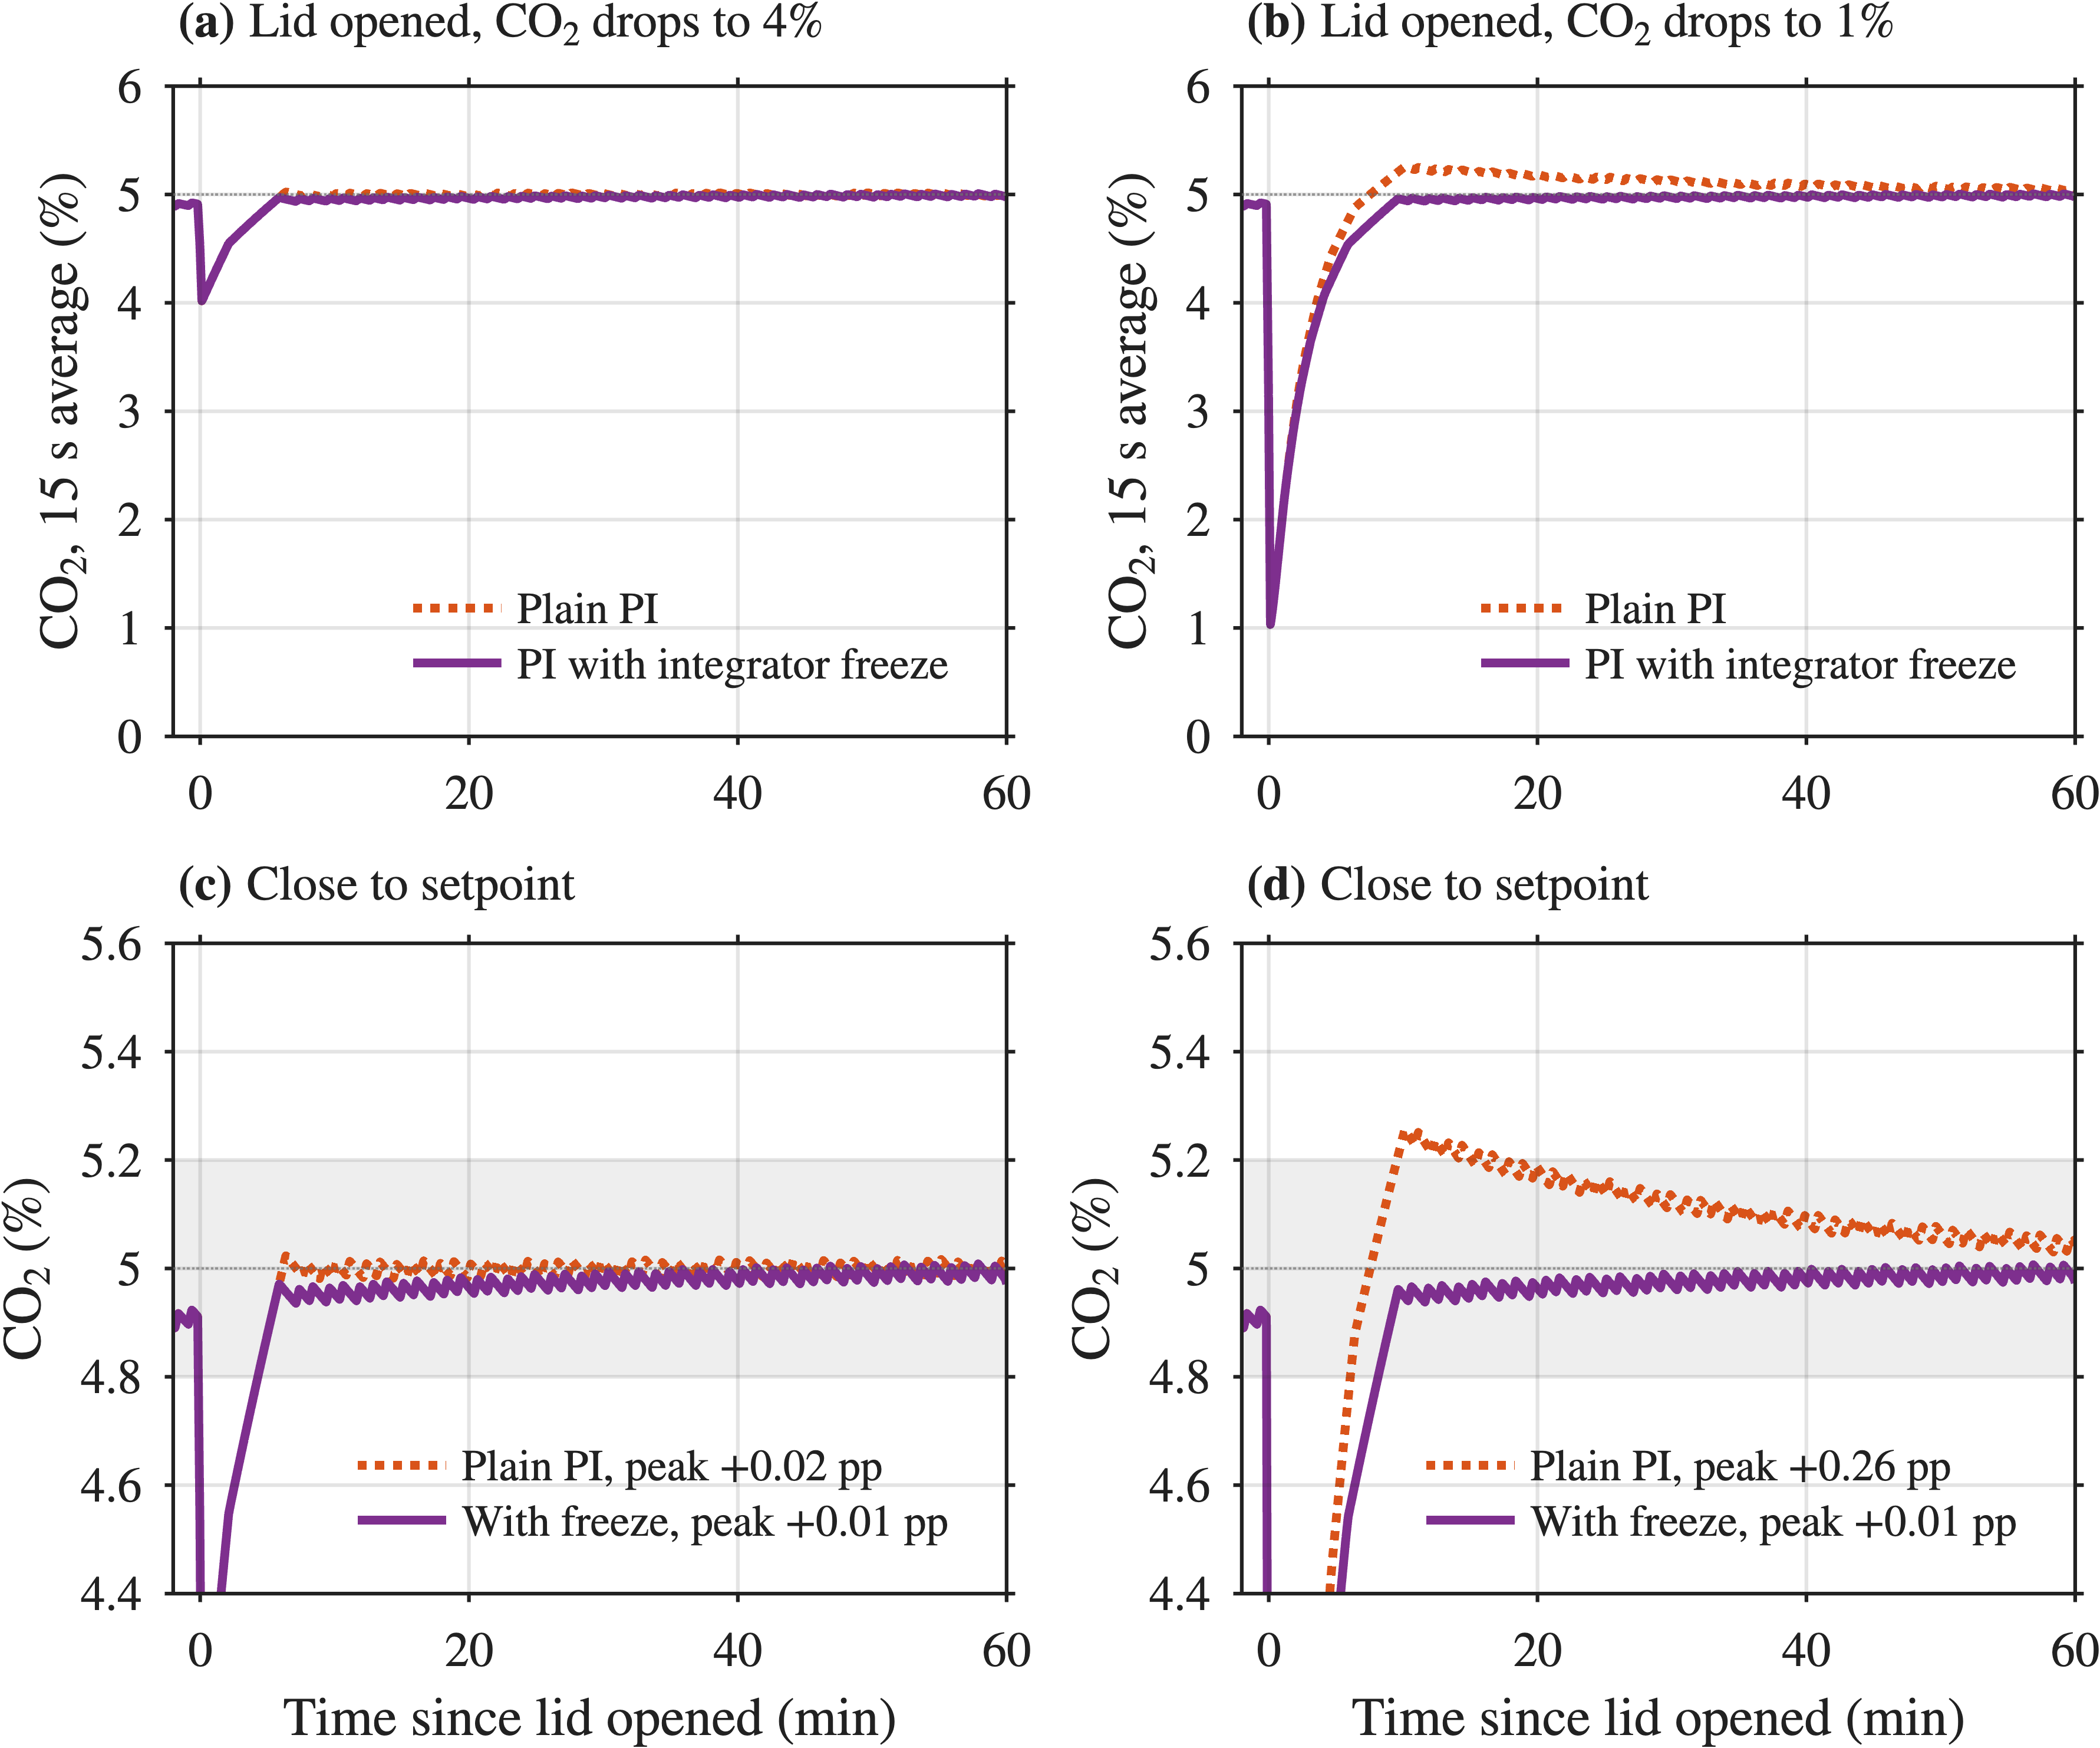
\includegraphics[width=0.74\textwidth,height=0.62\textheight,keepaspectratio]{figs/ch8/NEW_fig_C4_lid_openings.png}
    \caption[Recovery after a lid opening]{\textbf{Recovery after a lid opening,} with and without the integrator freeze, for drops to 4 and 1\,\%.}
    \label{fig:co2-lid}
\end{figure}

\begin{figure}[htbp]
    \centering
    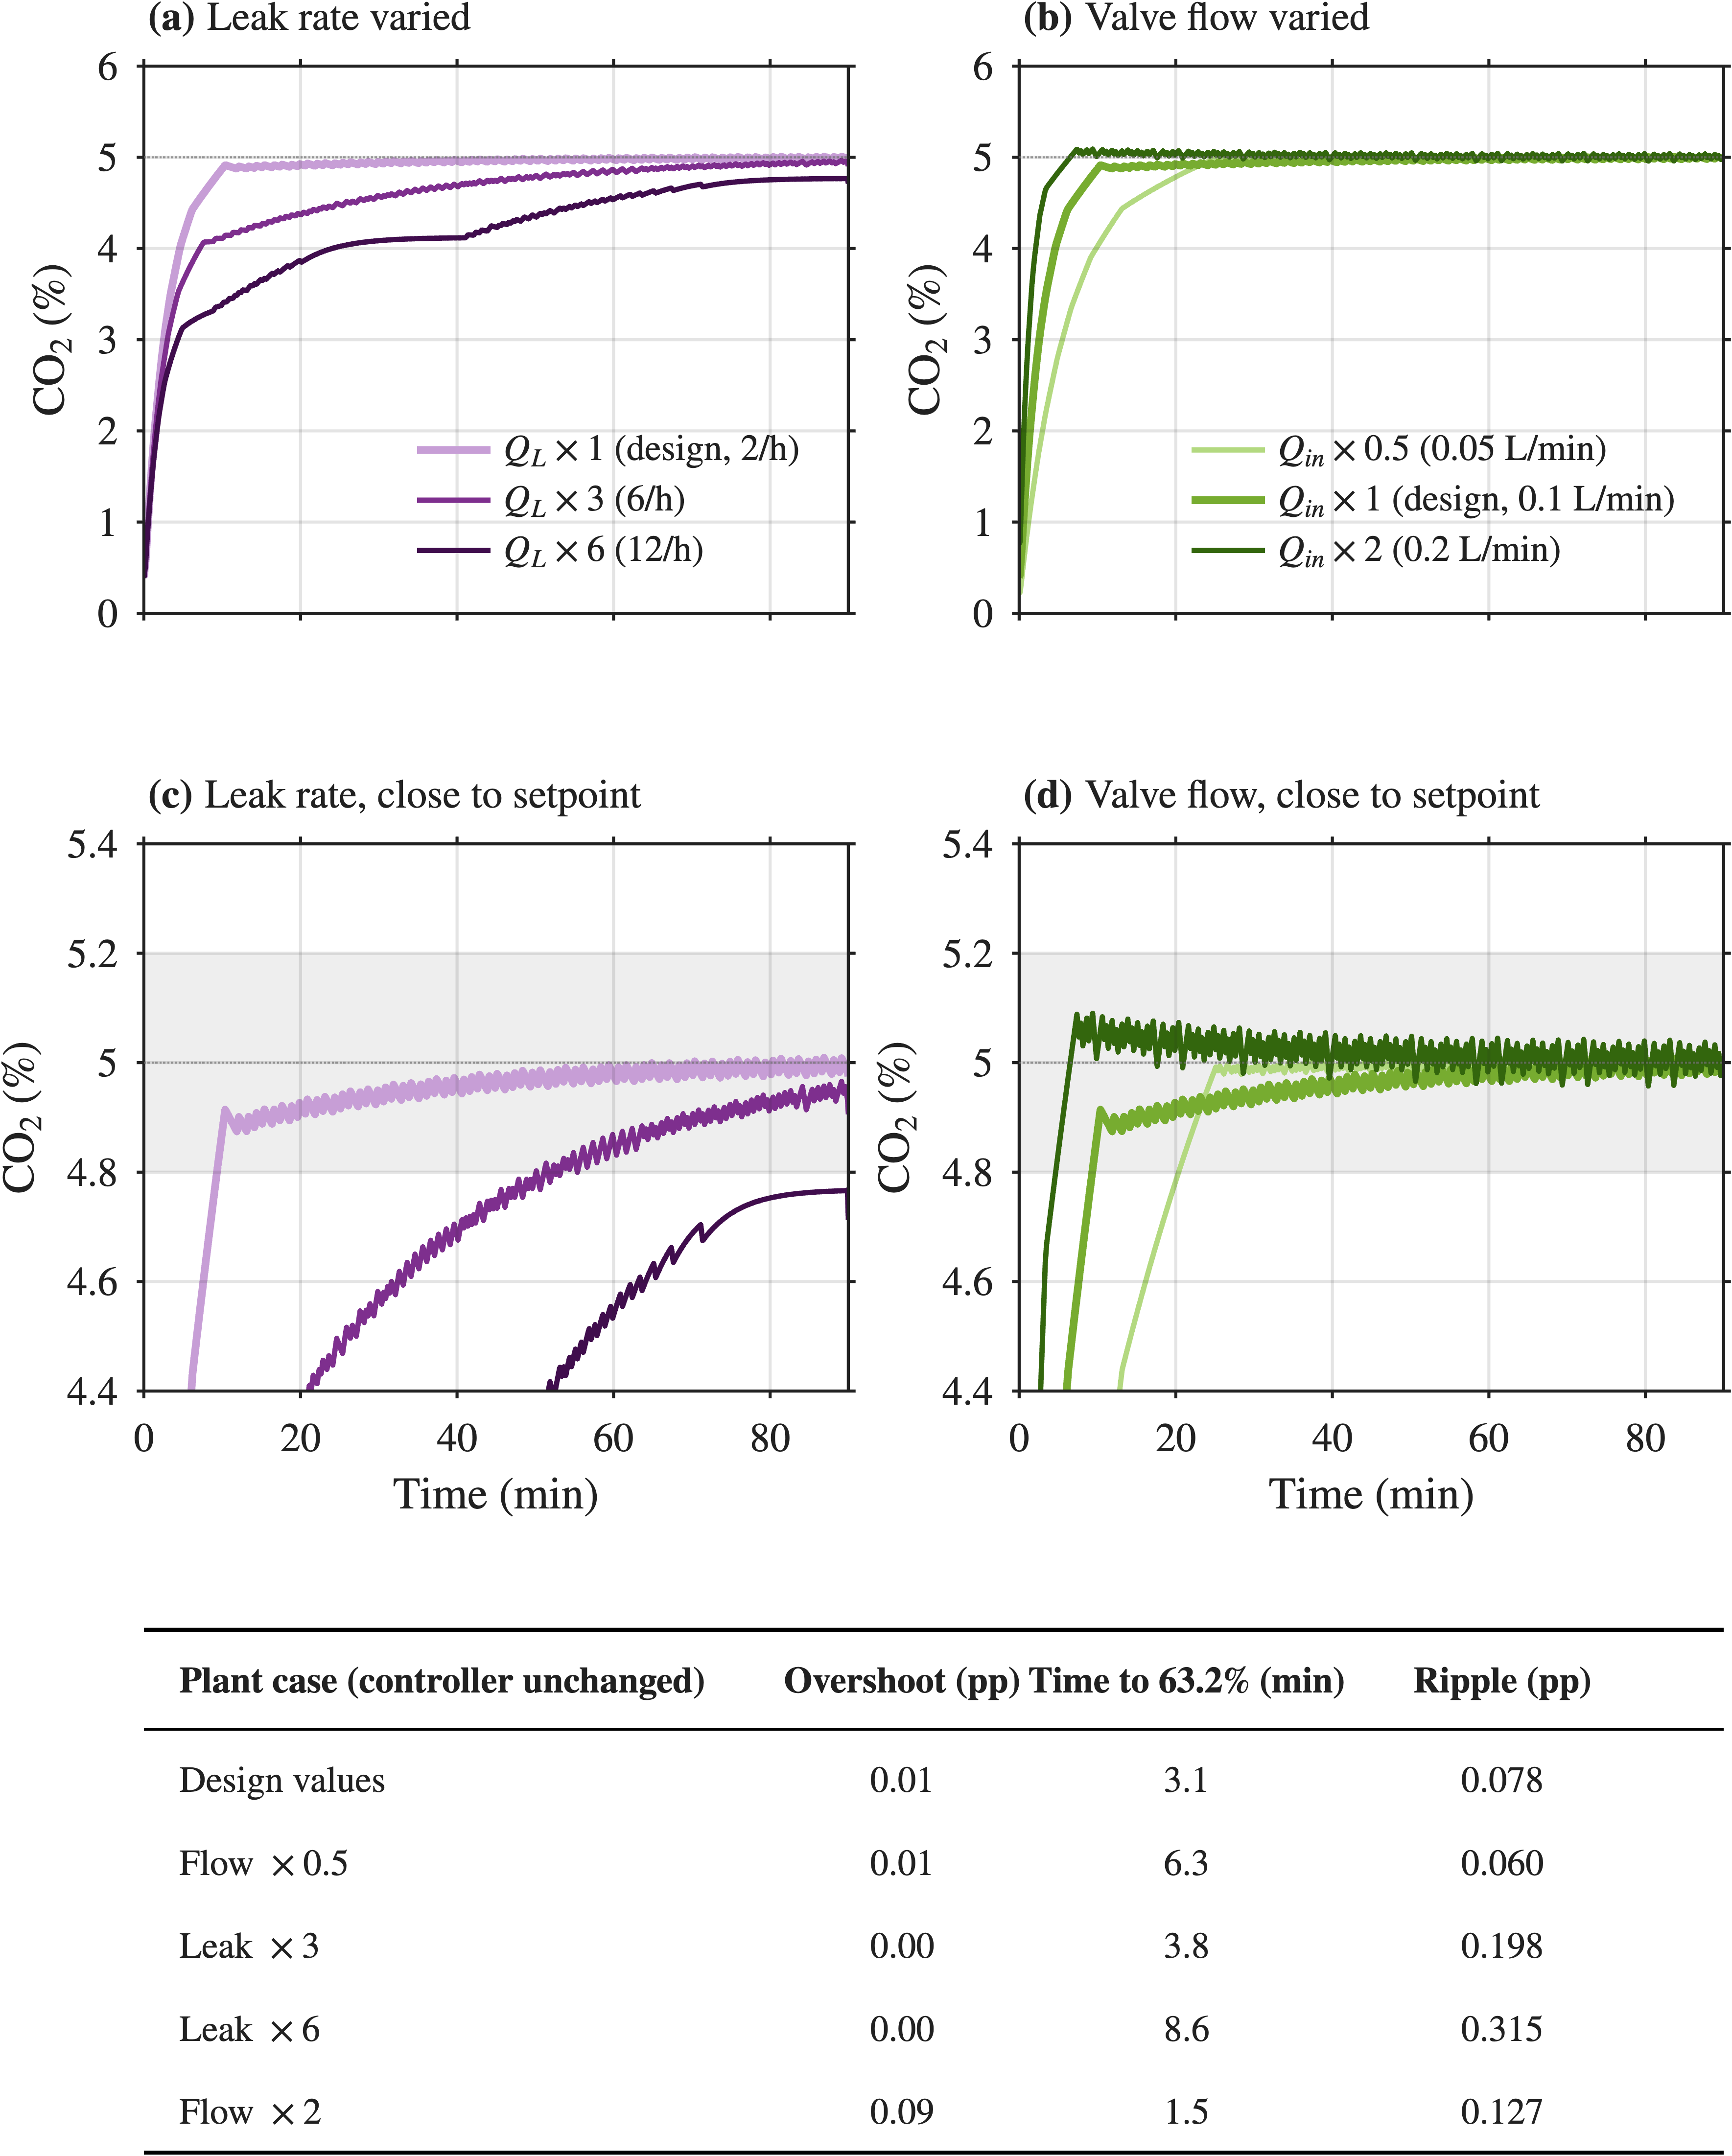
\includegraphics[width=0.74\textwidth,height=0.62\textheight,keepaspectratio]{figs/ch8/NEW_fig_C5_robustness.png}
    \caption[CO\textsubscript{2} loop robustness]{\textbf{Fill from room air with the leak and the flow varied,} controller unchanged.}
    \label{fig:co2-robustness}
\end{figure}

\begin{figure}[htbp]
    \centering
    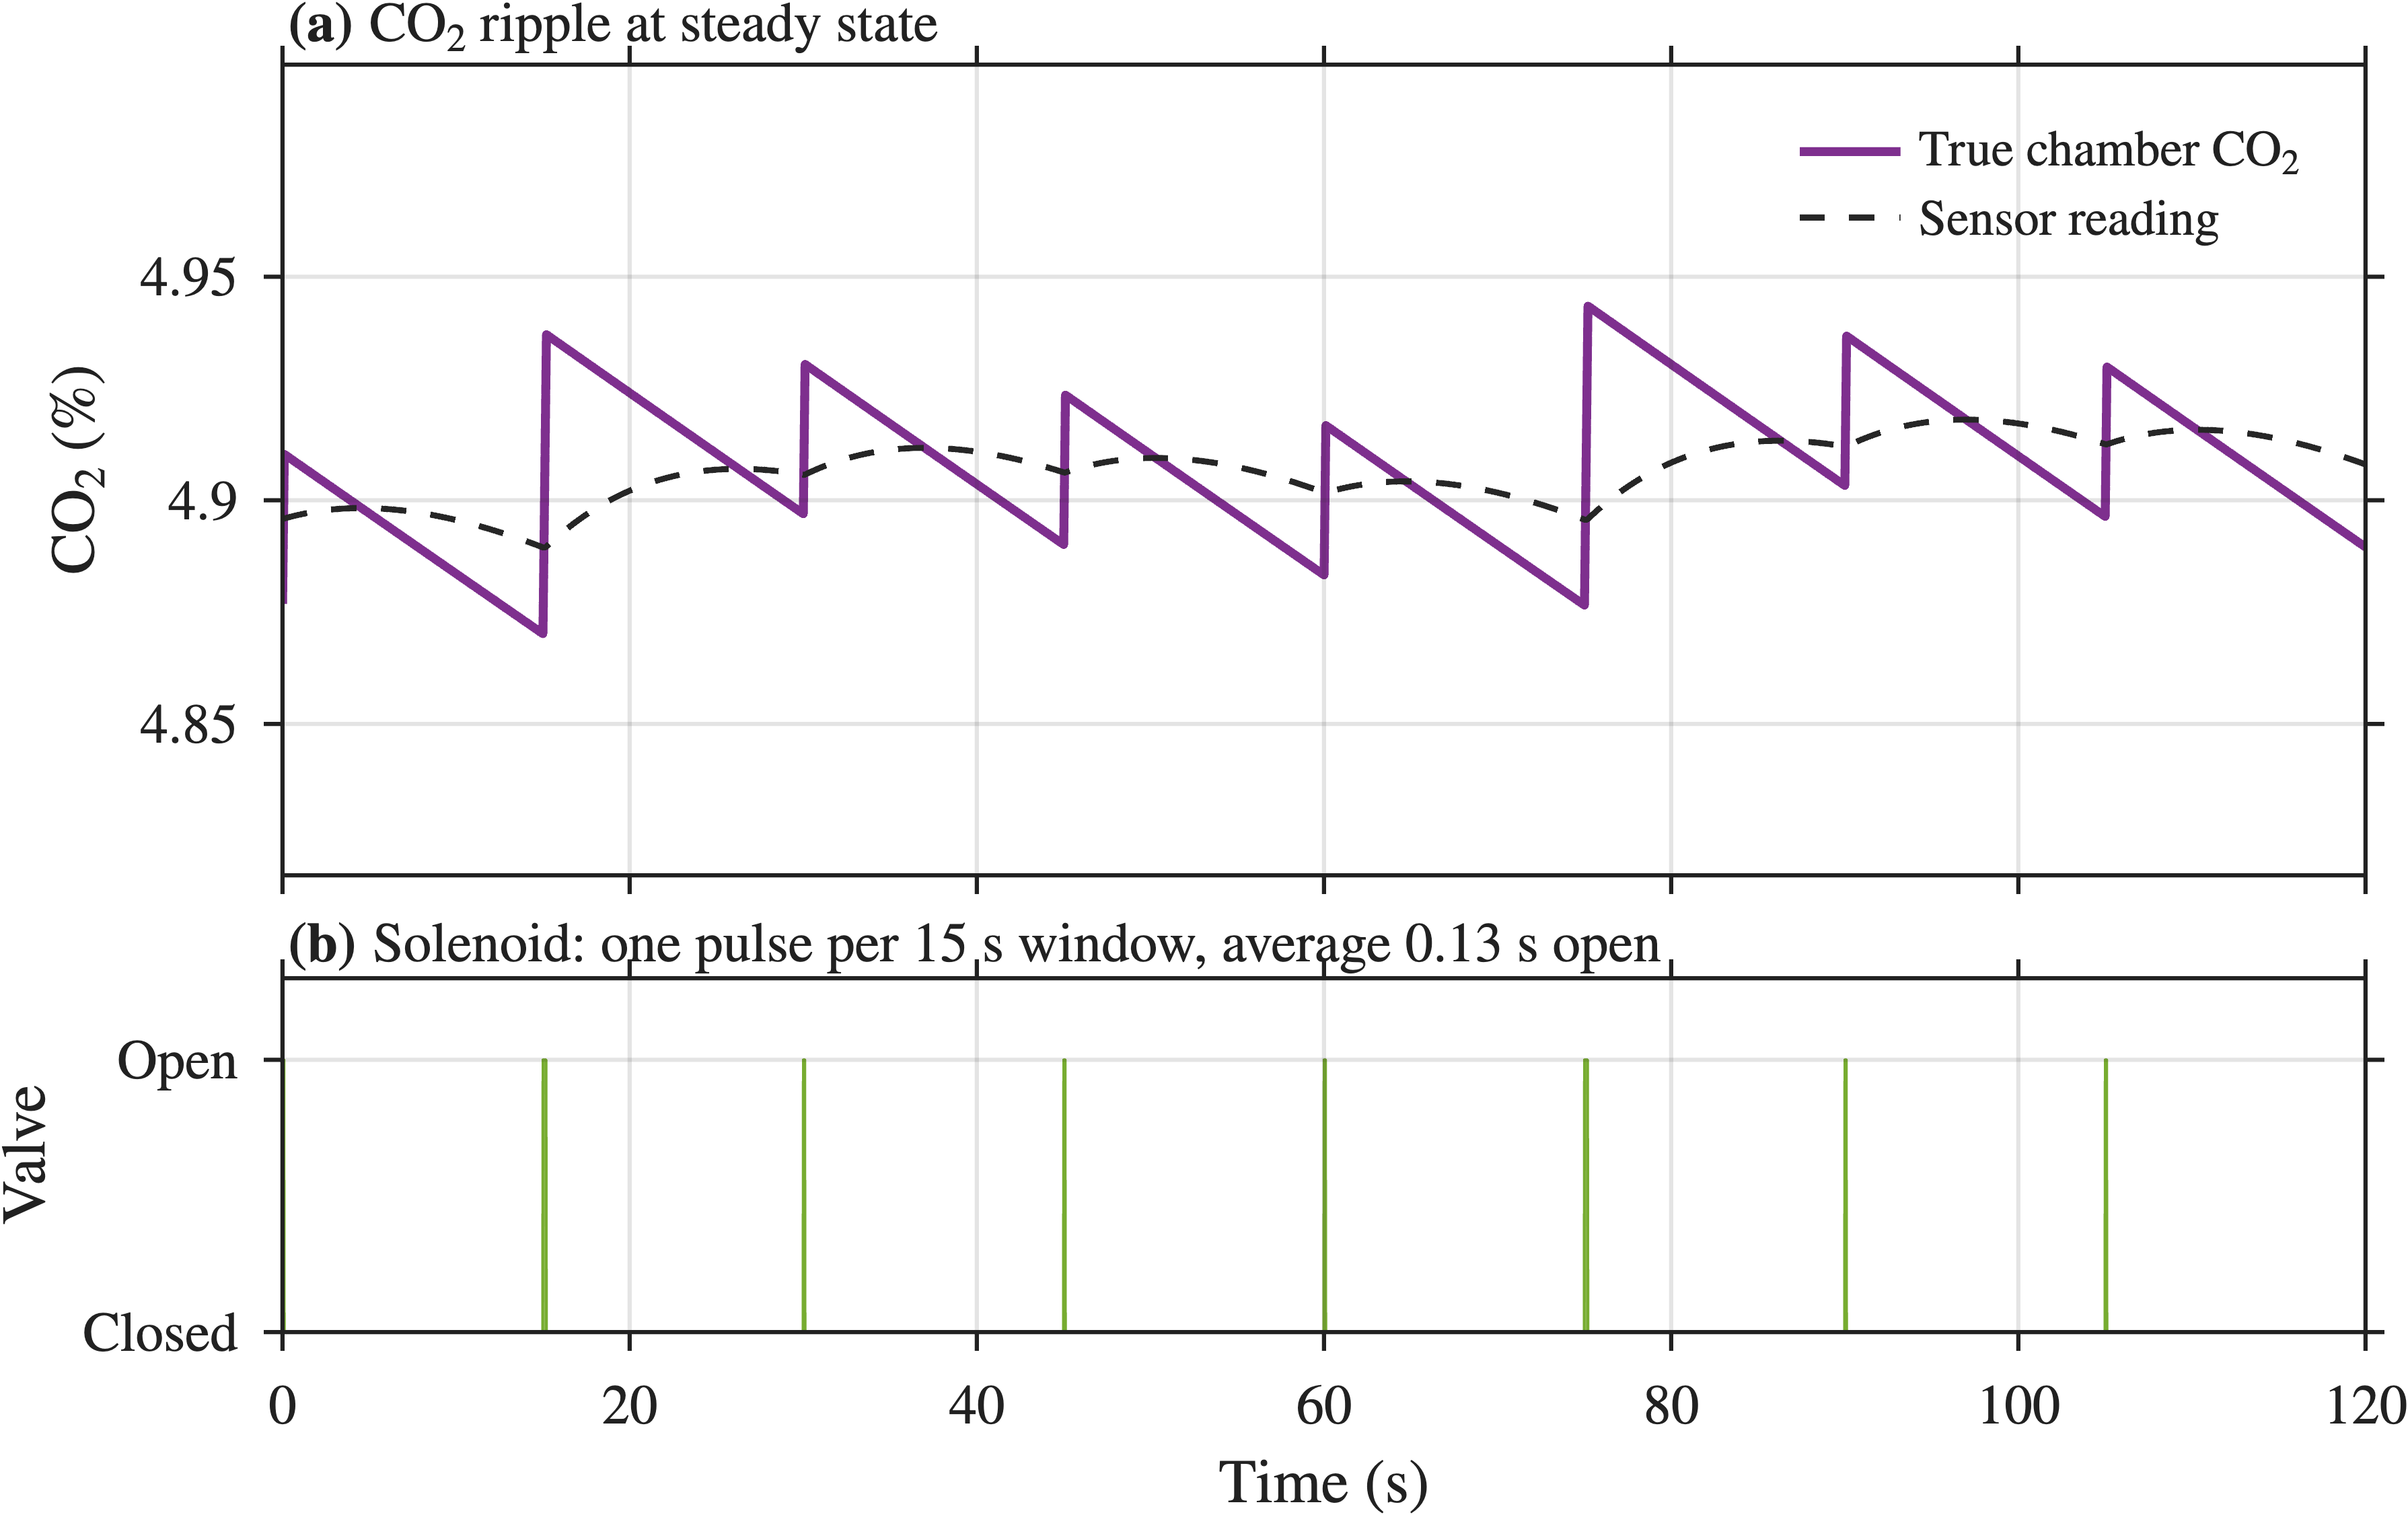
\includegraphics[width=0.74\textwidth,height=0.62\textheight,keepaspectratio]{figs/ch8/NEW_fig_C6_valve_pulses.png}
    \caption[Solenoid pulses at steady state]{\textbf{Solenoid pulses and the resulting ripple at steady state.} Average open time is 0.13\,s against a 0.1\,s minimum pulse.}
    \label{fig:co2-pulses}
\end{figure}

\begin{figure}[htbp]
    \centering
    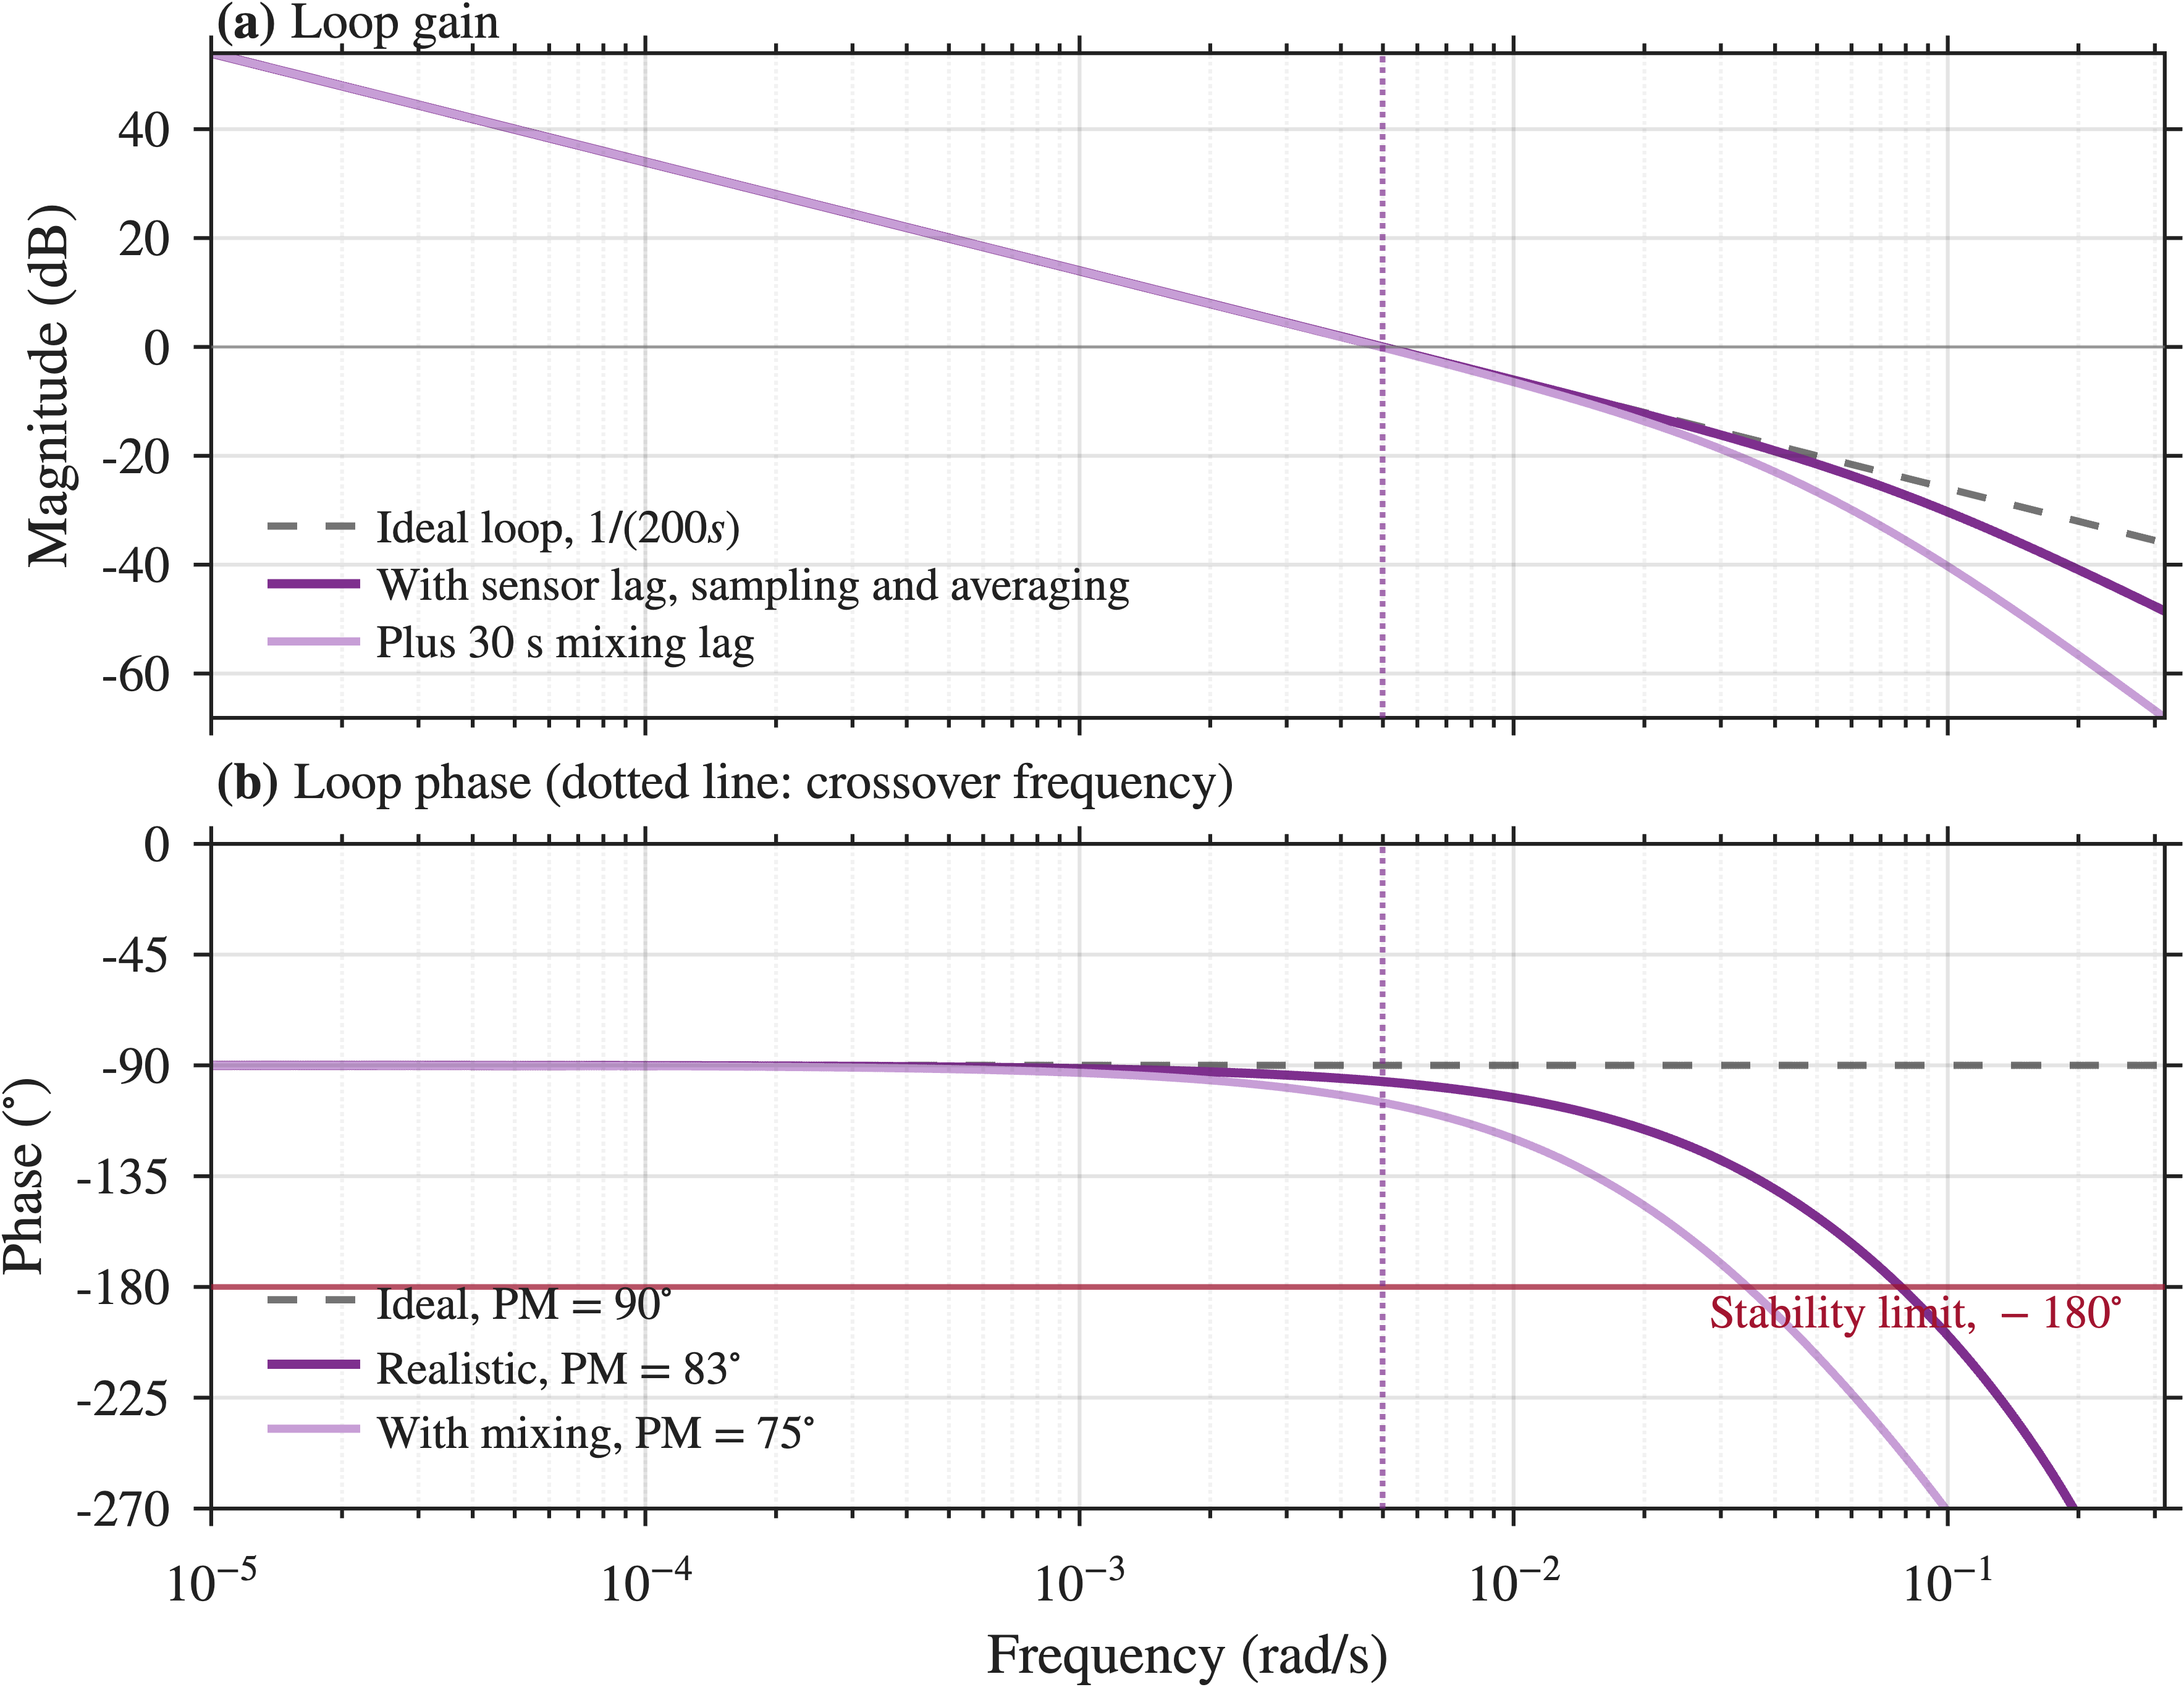
\includegraphics[width=0.74\textwidth,height=0.62\textheight,keepaspectratio]{figs/ch8/NEW_fig_C7_bode.png}
    \caption[CO\textsubscript{2} loop frequency response]{\textbf{Loop gain and phase,} ideal, with sensor lag and sampling, and with a 30\,s mixing delay added.}
    \label{fig:co2-bode}
\end{figure}
